\chapter{Evaluation}
\label{chap:evaluation}

\autoref{chap:sysmodel} defined the crash-aware system conceptually, and \autoref{chap:implementation} mapped it onto the Veins/\gls{inet} artifact.
This chapter asks whether that realization works as intended: does crash-triggered Voice traffic obtain better wireless service than ordinary Best Effort under contention, and what cost does that protection impose on ordinary traffic?

The evaluation is a protection-versus-cost study, not a claim of deterministic real-time guarantees~\cite{kosekszott2012What,IEEE80211e_2005}.
Two highway-density packages are used: a light-density sensitivity sweep (10~vehicles) and a heavy-density congestion stress case (100~vehicles), with emphasis on the latter~\cite{aguiar2026_veins_qos}.
Numeric bindings for timing, radio, load, and \gls{mac} policies are those of \autoref{tab:impl:parameters}; this chapter reports outcomes, not module wiring.

The chapter is organized as follows.
Section~\ref{sec:eval:setup} states the experimental matrix and seed budgets.
Section~\ref{sec:eval:metrics} defines metrics and aggregation.
Section~\ref{sec:eval:headline} states the headline answer and the two enabling conditions.
Section~\ref{sec:eval:hotspot} presents the primary positive result: Voice recovery under \texttt{hotspot\_high}.
Section~\ref{sec:eval:light} records the uniform-load null case that makes that result conditional.
Section~\ref{sec:eval:cost} prices the Best Effort cost of protection.
Section~\ref{sec:eval:discussion} discusses interpretation, practical significance, and limitations.
Section~\ref{sec:eval:summary} summarizes the conditional takeaway.

%%%%%%%%%%%%%%%%%%%%%%%%%%%%%%%%%%%%%%%%%%%%%%%%%%%%%%%%%%%%%%%%%%%%%%%%%%%%%%%%
\section{Experimental Setup}
\label{sec:eval:setup}

All experiments use the consolidated bindings in \autoref{tab:impl:parameters} and the reproducibility scripts in the public artifact~\cite{aguiar2026_veins_qos}.
Both density packages run the full matrix of five \gls{mac} policies and three offered-load profiles (15~configurations) with three OMNeT++ repetitions numbered \texttt{\#0}--\texttt{\#2}.
Each configuration name follows \texttt{<policy>\_netload\_<low|medium|high>} as documented in \autoref{chap:implementation}.
Simulation outputs and the scripts that regenerate the tabulated \glspl{kpi} are released with the public artifact~\cite{aguiar2026_veins_qos}.
A second matrix replays the same fifteen configurations under a hotspot overlay that concentrates Best Effort airtime near the crash source (15~configurations $\times$ 3~seeds $=$ 45~seeded runs; \autoref{sec:eval:hotspot}).

Contention is induced by offered load and fleet density rather than by synthetic random-waypoint mobility alone~\cite{veins_sommer2011}.
Best Effort inter-arrivals are Poisson: each vehicle redraws an exponential interval with the configured mean before every packet (\SI{500}{\milli\second}/\SI{250}{\milli\second}/\SI{125}{\milli\second} at low/medium/high).
At \texttt{netload\_high} that mean approaches 800~packets/s fleet-wide once all one hundred vehicles have entered; SUMO injects the fleet progressively, so the realized offer in these traces is about 22~thousand Best Effort transmissions per heavy run.
The crash source adds overlapping Voice repeats during the alert window (eight physical copies, \SI{5}{\milli\second} gap at high load), a sustained stream of roughly 400~physical packets/s while the window is active.
With a genuine Poisson offer the channel does \emph{not} enter queue overflow: Best Effort P95 stays sub-millisecond under plain \gls{dcf} and EDCA, and overflow counters remain zero.
The policy contrast under that uniform offer is therefore Best Effort cost, not a Voice-tail race under saturation~\cite{aguiar2026_veins_qos,Continuous_Backoff_Freezing_Li}.

%%%%%%%%%%%%%%%%%%%%%%%%%%%%%%%%%%%%%%%%%%%%%%%%%%%%%%%%%%%%%%%%%%%%%%%%%%%%%%%%
\section{Metrics and Aggregation}
\label{sec:eval:metrics}

The primary metrics are class-specific end-to-end delay, jitter, multicast reach, and \gls{mac}-layer losses; the definitions below apply to the Evaluation tables in this chapter.

End-to-end delay runs from packet creation to reception at each receiving vehicle.
Best Effort stamps creation at each physical send.
Crash Voice stamps creation at the logical burst start, so Voice delay is \emph{alert age}: time from the first attempt of a sequence until a receiver's first accepted copy, including any wait for a later physical repeat when earlier copies miss.
Mean delays aggregate per-run statistics across receivers, while tail and jitter statistics pool all receivers' per-packet samples, excluding locally looped-back copies.
The \gls{p95} is the main tail metric; mean absolute jitter summarizes short-term delay variation on the same samples.
A crash-node Best Effort slice records delay only for Best Effort packets whose source is the designated crash vehicle, so Voice can be compared with Best Effort from the same sender rather than with the fleet average.

Because every packet is multicast, reception is a fan-out that can exceed one:
Voice \emph{RX/alert} divides received alert copies by logical alert sequences;
Best Effort \emph{RX/TX} divides received background copies by transmitted packets.
\gls{mac} analysis reports total drops, drops per application transmission, and per-access-category attribution (Best Effort, Voice, unclassified); the Voice-attributed drop count quantifies crash-frame loss at the \gls{mac} layer, summed over all nodes and including receive-side discards of corrupted frames.
When the per-category counters sum to twice the aggregate drop counter, the analysis pipeline halves the attributed counts so that categories sum to the aggregate (a double-counting guard in the parser); attribution is unavailable under \texttt{plain}, where no classifier assigns access categories.
Controller instrumentation adds Voice protection activations, Best Effort drops while blocked, and held Best Effort grants (\autoref{chap:implementation}).

Each repetition yields one run-level \gls{kpi} row.
Configuration summaries in this chapter are arithmetic means over seeds; tail statistics are computed per run over the pooled receiver samples and then averaged across seeds (a mean of per-run percentiles).
Headline delay, jitter, and reach tables also report the minimum--maximum range across those seeds.
Both densities use three seeds; \emph{no significance tests are reported}.
The numbers are therefore qualitative mechanism checks under a controlled matrix, not proven effect sizes~\cite{aguiar2026_veins_qos}.
Unless noted otherwise, relative improvements are versus \texttt{plain}; Voice-attributed \gls{mac}-drop comparisons use EDCA because \texttt{plain} has no access-category attribution.

%%%%%%%%%%%%%%%%%%%%%%%%%%%%%%%%%%%%%%%%%%%%%%%%%%%%%%%%%%%%%%%%%%%%%%%%%%%%%%%%
\section{Voice Protection Under Load: The Headline Answer}
\label{sec:eval:headline}

Does crash-triggered Voice traffic obtain better wireless service than ordinary Best Effort under contention?
The answer from the full matrix is conditional: emergency preemption recovers Voice service only when (i)~near-crash airtime is concentrated in a few senders and (ii)~the alert burst cadence is dense enough to keep protection armed for most of the crash window.
\autoref{tab:eval:glance} maps the headline cells; \autoref{fig:eval:regime_contrast} plots the same regime contrast.

At heavy \texttt{netload\_high} every policy sits near 2.2~ms Voice P95---a floor imposed by the \SI{2}{\milli\second} per-copy dispatch jitter of the alert generator rather than by channel access; the low and medium profiles, whose jitter is \SI{5}{\milli\second}, sit near 4.6--4.9~ms instead (\autoref{sec:eval:light}).
Under \texttt{hotspot\_high} only emergency compresses the inflated tail.
Protection is therefore an event-triggered escalation whose gain is set by channel geometry and burst cadence, not an always-on Voice accelerator.
Section~\ref{sec:eval:hotspot} develops the positive cell; Section~\ref{sec:eval:light} records the uniform null; Section~\ref{sec:eval:cost} prices the Best Effort bill.

\begin{table}[htb]
	\ABNTEXfontereduzida
	\caption{\label{tab:eval:glance}Results at a glance (heavy density, three-seed means). Relative Voice gains are versus \texttt{plain}. Detail tables follow in the sections named in the last column.}
	\begin{center}
		\small
		\setlength{\tabcolsep}{3pt}
		\begin{tabular}{@{}llp{0.35\linewidth}l@{}}
			\toprule
			\textbf{Cell} & \textbf{Voice P95} & \textbf{Main contrast} & \textbf{Where} \\
			\midrule
			Uniform \texttt{netload\_high} &
			  $\approx$2.2~ms, all policies &
			  No Voice win; Best Effort cost &
			  \autoref{sec:eval:light} \\
			Hotspot \texttt{hotspot\_high} &
			  $\approx$18.5~$\rightarrow$~14.6~ms &
			  Emergency: $-39\%$ mean / $-21\%$ P95 &
			  \autoref{sec:eval:hotspot} \\
			Hotspot \texttt{medium}/\texttt{low} &
			  No Voice gain &
			  Sparse bursts fail the arming condition &
			  \autoref{sec:eval:hotspot:dose} \\
			Emergency BE drops &
			  --- &
			  $\approx 16.1\times10^{3}$ (hotspot) vs $\approx 2.5\times10^{3}$ (uniform) &
			  \autoref{sec:eval:cost} \\
			\bottomrule
		\end{tabular}
	\end{center}
	\fonte{Prepared by the author.}
\end{table}

\begin{figure}[htb]
	\caption{\label{fig:eval:regime_contrast}Voice P95 delay by policy at high load under uniform Poisson offer versus hotspot contention (100~vehicles, three-seed means). Protection is inert under diffuse load and selective under concentrated near-crash airtime: only emergency compresses the hotspot tail. Here and in the remaining figures the baseline policy is labelled \texttt{DCF}; the tables call the same policy \texttt{plain}.}
	\begin{center}
		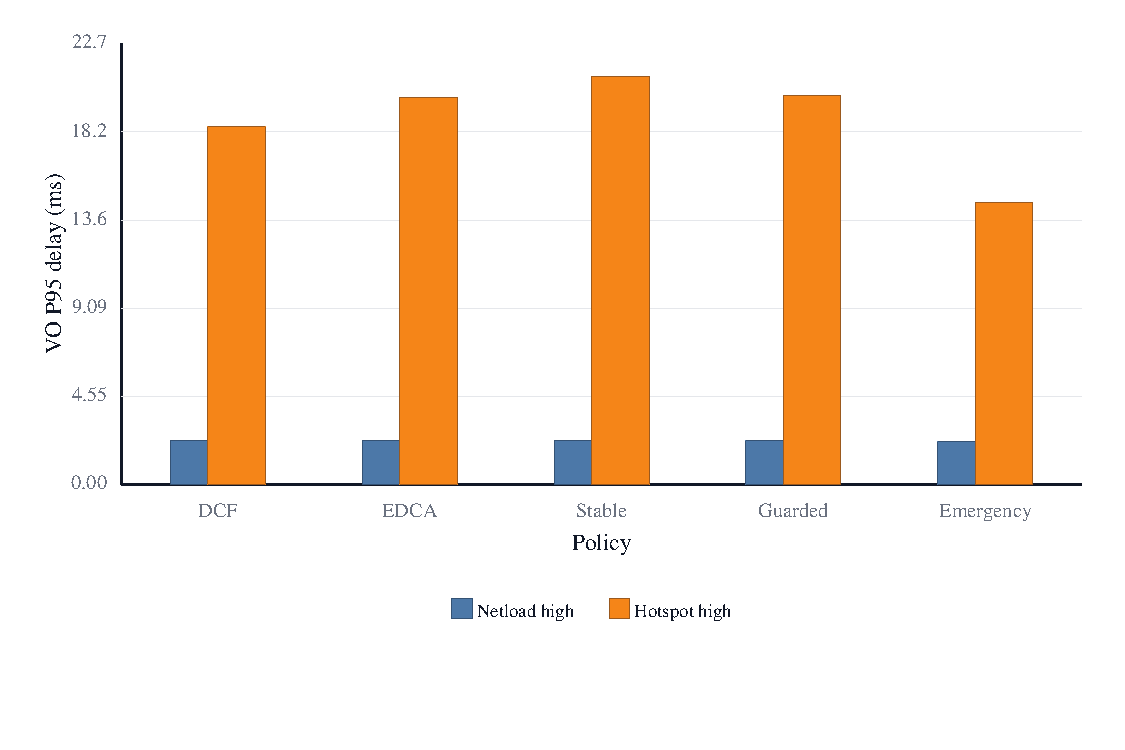
\includegraphics[width=0.95\linewidth, trim=0 50 0 8, clip]{Figs/fig_10_regime_vo_p95_contrast_highway_heavy.pdf}
	\end{center}
	\fonte{Prepared by the author.}
\end{figure}

%%%%%%%%%%%%%%%%%%%%%%%%%%%%%%%%%%%%%%%%%%%%%%%%%%%%%%%%%%%%%%%%%%%%%%%%%%%%%%%%
\section{Hotspot Load: Voice Recovery Under Concentrated Contention}
\label{sec:eval:hotspot}

Under a uniform Poisson offer, near-crash collision opportunities are diffuse across about one hundred senders, so node-local Best Effort suppression removes a negligible share of ambient airtime and can fire only after a first Voice copy was decoded (\autoref{sec:eval:light}).
The enabling contraposition is concentrated airtime: if a few crash-adjacent senders dominate the channel, suppression acquires a target and a Voice effect should appear.

The hotspot overlay \texttt{\_hotspot3} (\autoref{sec:impl:matrix}) implements that regime.
The three vehicles entering the corridor immediately after the crash node bulk-upload about \SI{2.4}{\mega\bit\per\second} each for the whole run, roughly tripling aggregate Best Effort transmissions per run from $22\times10^{3}$ to $72\times10^{3}$.
That higher offer pushes Voice-attributed \gls{mac} losses from about $3.7\times10^{3}$ under uniform \texttt{netload\_high} to about $25\times10^{3}$ under hotspot EDCA \emph{before} policies separate.
The crash source, the alert window, and every metric definition are unchanged; configurations are named \texttt{<policy>\_hotspot\_<profile>}.

\subsection{The \texttt{hotspot\_high} cell}
\label{sec:eval:hotspot:high}

\autoref{tab:eval:hotspot} and \autoref{fig:eval:hotspot_delay} report the dense-burst high-load cell---the only hotspot cell where Voice delay is policy-sensitive.
Plain \gls{dcf} and plain EDCA reach Voice P95 of 18.5--20~ms.
Emergency holds the same tail at 14.6~ms and the Voice mean at 2.78~ms ($-39\%$ mean and $-21\%$ P95 versus plain; $-38\%$ / $-27\%$ versus EDCA).
Voice-attributed collision losses fall from $25.2\times10^{3}$ to $17.8\times10^{3}$ ($-30\%$ versus EDCA), and the three-seed P95 ranges do not overlap the baselines'.
Emergency lowers both central tendency and tail, but P95 remains an order of magnitude above the mean because alert age is dominated by occasional late first-copy successes under collision-heavy windows.
The mechanism is visible in the controller counters: under the 20~ms $\times$~8-copy alert stream the blocked duty cycle is near-continuous---about $16.1\times10^{3}$ Best Effort frames are dropped while blocked (\autoref{tab:eval:hotspot})---so the hot queues never refill the arena during the window.
Multicast reach remains geometry-limited at about ten receivers per alert for every policy: protection buys latency and integrity, not fan-out.

\begin{table}[H]
	\ABNTEXfontereduzida
	\caption{\label{tab:eval:hotspot}Hotspot high-load Voice protection results (100~vehicles, hotspot nodes 1--3 streaming 1200~B, three-run means). \emph{VO \glsentryshort{mac} drops} are Voice-attributed incorrectly-received counts summed over nodes; \emph{\glsentryshort{be} from crash} is the same-sender Best Effort mean delay (starvation under EDCA/\texttt{stable}/\texttt{guarded}); \emph{\glsentryshort{be} dropped blocked} counts emergency preemptions.}
	\begin{center}
		\scriptsize
		\setlength{\tabcolsep}{3.5pt}
		\resizebox{\linewidth}{!}{%
		\begin{tabular}{@{}lrrrrrr@{}}
			\toprule
			\textbf{Policy} &
			\textbf{VO mean (ms)} &
			\textbf{VO P95 (ms)} &
			\textbf{VO RX/alert} &
			\textbf{VO MAC drops ($\times 10^{3}$)} &
			\textbf{\gls{be} from crash (ms)} &
			\textbf{\gls{be} dropped blocked ($\times 10^{3}$)} \\
			\midrule
			Plain     & 4.540 & \shortstack{18.45\\[-1pt]{\scriptsize [16.1--19.9]}} & 9.670 & n.a. & 1.548 & 0 \\
			EDCA      & 4.448 & \shortstack{19.96\\[-1pt]{\scriptsize [18.7--20.7]}} & 9.624 & 25.2 & \shortstack{1453\\[-1pt]{\scriptsize (1.45~s)}} & 0 \\
			Stable    & 4.608 & \shortstack{21.04\\[-1pt]{\scriptsize [18.8--22.8]}} & 9.636 & 25.4 & \shortstack{1386\\[-1pt]{\scriptsize (1.39~s)}} & 0 \\
			Guarded   & 4.439 & \shortstack{20.04\\[-1pt]{\scriptsize [19.8--20.4]}} & 9.689 & 25.1 & \shortstack{981\\[-1pt]{\scriptsize (0.98~s)}} & 0 \\
			Emergency & \textbf{2.781} & \textbf{\shortstack{14.56\\[-1pt]{\scriptsize [11.8--16.0]}}} & \textbf{9.835} & \textbf{17.8} & 3.335 & 16.1 \\
			\bottomrule
		\end{tabular}%
		}
	\end{center}
	\fonte{Prepared by the author.}
\end{table}

\begin{figure}[htb]
	\caption{\label{fig:eval:hotspot_delay}Voice mean and P95 delay by policy at \texttt{hotspot\_high} (100~vehicles). Only emergency, whose preemption keeps hot Best Effort queues out of the collision arena, compresses the tail that hotspot contention inflates.}
	\begin{center}
		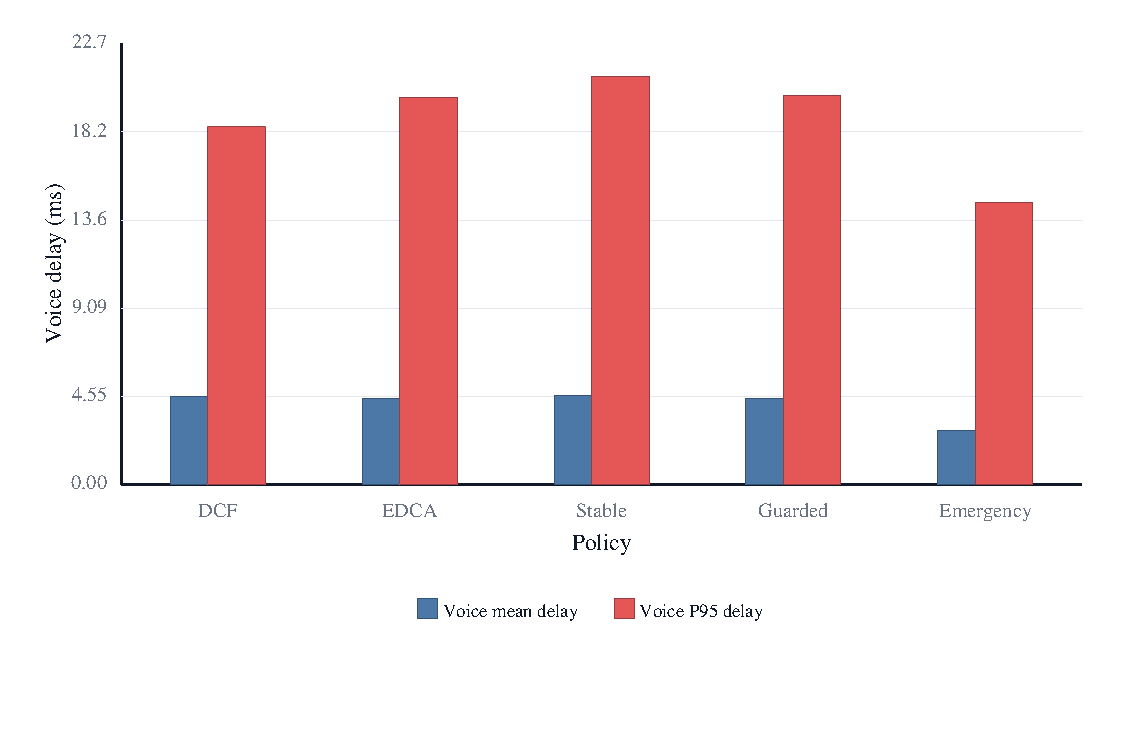
\includegraphics[width=0.95\linewidth, trim=0 50 0 8, clip]{Figs/fig_08_hotspot_vo_delay_by_policy_highway_heavy.pdf}
	\end{center}
	\fonte{Prepared by the author.}
\end{figure}

Dropping, not deferring, is the load-shedding step that matters under concentrated contention.
\texttt{stable} and \texttt{guarded} keep Voice P95 on the EDCA baseline (20--21~ms): blocking without dropping never clears the hot queues.
The same policies starve the crash node's own Best Effort stream---delivered packets from that sender average $0.98$--$1.45$~\si{\second} of queueing delay---whereas emergency and plain keep that same-sender slice at 3.3~ms and 1.5~ms respectively (\autoref{tab:eval:hotspot}).
Preemption therefore doubles as a starvation cure for the alerted node: it is what both recovers Voice and keeps the sender's ordinary traffic responsive when continuous hotspot demand would otherwise own the local arbitration forever.

\subsection{Dose response: why only dense bursts win}
\label{sec:eval:hotspot:dose}

The Voice gain is conditional on burst density (\autoref{tab:eval:hotspot_dose}, \autoref{fig:eval:hotspot_dose}).
At \texttt{hotspot\_high} the 20~ms period with eight copies keeps protection armed for most of the crash window.
At \texttt{medium} (75~ms, four copies) and \texttt{low} (120~ms, three copies) the blocked duty cycle falls to roughly one third or less, hot traffic refills the gaps between blocks, and emergency becomes neutral-to-harmful on the Voice mean ($+10\%$ and $+16\%$ respectively).
Voice service therefore appears only when \emph{both} enabling conditions hold: concentrated near-crash airtime \emph{and} a cadence dense enough to cover it.

\begin{table}[htb]
	\ABNTEXfontereduzida
	\caption{\label{tab:eval:hotspot_dose}Dose response of emergency against plain under hotspot load (three-run means). Voice gains appear only where the burst cadence keeps protection armed for most of the crash window.}
	\begin{center}
		\small
		\setlength{\tabcolsep}{5pt}
		\begin{tabular}{@{}llrr@{}}
			\toprule
			\textbf{Load} & \textbf{Burst profile} & \textbf{$\Delta$ VO mean} & \textbf{$\Delta$ VO P95} \\
			\midrule
			\texttt{high}   & 20~ms $\times$ 8 copies & $-39\%$ & $-21\%$ \\
			\texttt{medium} & 75~ms $\times$ 4 copies & $+10\%$ & $+5\%$ \\
			\texttt{low}    & 120~ms $\times$ 3 copies & $+16\%$ & $+0\%$ \\
			\bottomrule
		\end{tabular}
	\end{center}
	\fonte{Prepared by the author.}
\end{table}

\begin{figure}[htb]
	\caption{\label{fig:eval:hotspot_dose}Voice P95 delay across offered-load profiles under hotspot load (100~vehicles), plain versus emergency (three-seed means). Protection differentiates only at \texttt{high}, where dense bursts keep Best Effort suppression armed for most of the crash window.}
	\begin{center}
		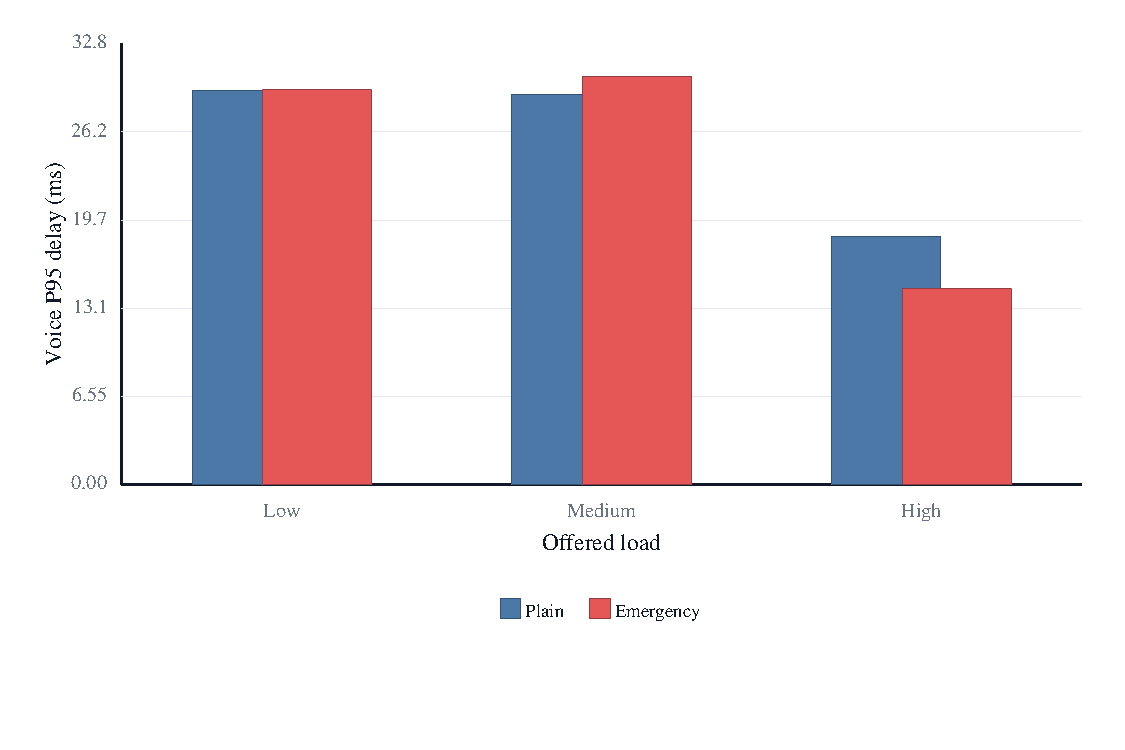
\includegraphics[width=0.95\linewidth, trim=0 50 0 8, clip]{Figs/fig_09_hotspot_vo_p95_by_load_highway_heavy.pdf}
	\end{center}
	\fonte{Prepared by the author.}
\end{figure}

%%%%%%%%%%%%%%%%%%%%%%%%%%%%%%%%%%%%%%%%%%%%%%%%%%%%%%%%%%%%%%%%%%%%%%%%%%%%%%%%
\section{Uniform Load: The Null Voice Case}
\label{sec:eval:light}

The uniform Poisson matrix is the scientific null against which \autoref{sec:eval:hotspot} is read.
With no concentrated near-crash sender, every policy keeps Voice alert age within a few tens of microseconds of plain \gls{dcf}; the policy contrast is Best Effort cost.

\subsection{Light-density gating numbers}
\label{sec:eval:light:gating}

\autoref{tab:eval:light} reports light-density high-load cells versus \texttt{plain\_netload\_high}.
Voice stays flat near 2.08~ms P95 (within $1.3\%$ of plain).
\texttt{stable} and \texttt{guarded} inflate Best Effort P95 from 0.44~ms to 49~ms and 9.0~ms; emergency shortens it to 0.37~ms by dropping stale Best Effort work rather than by protecting Voice.
The sweep is a gating test: adaptive blocking without dropping is already risky when protection windows can open under low channel stress.

\begin{table}[htb]
	\ABNTEXfontereduzida
	\caption{\label{tab:eval:light}Light-density high-load gating results versus \texttt{plain\_netload\_high} (10~vehicles, three-seed means). Voice columns are relative changes; Best Effort P95 is absolute (ms) so four-digit percentages do not dominate the table. Plain baselines (ms): Voice mean 0.786, Voice P95 2.078, Best Effort mean 0.383, Best Effort P95 0.437.}
	\begin{center}
		\setlength{\tabcolsep}{5pt}
		\begin{tabular}{@{}lrrr@{}}
			\toprule
			\textbf{Policy} &
			\textbf{VO mean} &
			\textbf{VO P95} &
			\textbf{BE P95 (ms)} \\
			\midrule
			Plain (baseline) & --- & --- & 0.44 \\
			EDCA      & $+1.3\%$  & $-0.0\%$   & 0.42 \\
			Stable    & $+0.9\%$  & $+0.5\%$  & 49 \\
			Guarded   & $-1.3\%$  & $-1.3\%$  & 9.0 \\
			Emergency & $+2.4\%$ & $+0.2\%$ & 0.37 \\
			\bottomrule
		\end{tabular}
	\end{center}
	\fonte{Prepared by the author.}
\end{table}

\subsection{Heavy-density confirmation}
\label{sec:eval:heavy:qos}

At one hundred vehicles the same null Voice story holds, only louder.
\autoref{tab:eval:heavy_qos} and \autoref{fig:eval:p95_gap_heavy} show Voice mean, P95, and jitter within a few tens of microseconds across all five policies (P95 2.21--2.25~ms).
EDCA does not lower Voice alert age relative to plain \gls{dcf}.
The policy contrast is Best Effort: \texttt{stable} raises fleet Best Effort P95 from 0.51~ms to 30~ms; \texttt{guarded} to 3.9~ms; emergency keeps 0.37~ms by preemption.
That lower emergency P95 is not better Best Effort service: delay is measured only on delivered packets, so dropping frames while blocked removes the slow tail from the sample while the cost appears as reach loss (Best Effort RX/TX falls from 8.06 under \texttt{plain} to 6.93).
Voice RX/alert is 9.95 for every policy (geometry-limited fan-out).
Voice-attributed \gls{mac} drops sit near $3.7\times10^{3}$ under every QoS-enabled policy and do not separate emergency from EDCA; Best Effort queue overflow is zero throughout.
Node-local suppression therefore has no Voice target under diffuse contention: it cannot change how many alerts arrive or how many collide.

\begin{table}[htb]
	\ABNTEXfontereduzida
	\caption{\label{tab:eval:heavy_qos}Heavy-density high-load delay, jitter, and multicast reach (100~vehicles, three-run means with min--max range across seeds; delays and jitter in~ms).}
	\begin{center}
		\small
		\setlength{\tabcolsep}{6pt}
		\begin{tabular}{@{}lrrrr@{}}
			\toprule
			\multicolumn{5}{@{}l}{\textit{\gls{vo} (crash alert)}} \\
			\midrule
			\textbf{Policy} & \textbf{Mean} & \textbf{P95} & \textbf{Jitter} & \textbf{RX/alert} \\
			\midrule
			Plain      & \shortstack{0.991\\[-1pt]{\scriptsize [0.975--1.021]}} & \shortstack{2.249\\[-1pt]{\scriptsize [2.229--2.287]}} & \shortstack{1.024\\[-1pt]{\scriptsize [1.010--1.044]}} & \shortstack{9.954\\[-1pt]{\scriptsize [8.743--10.843]}} \\
			EDCA       & \shortstack{0.994\\[-1pt]{\scriptsize [0.982--1.003]}} & \shortstack{2.242\\[-1pt]{\scriptsize [2.220--2.255]}} & \shortstack{1.018\\[-1pt]{\scriptsize [1.005--1.034]}} & \shortstack{9.954\\[-1pt]{\scriptsize [8.743--10.843]}} \\
			Stable     & \shortstack{0.988\\[-1pt]{\scriptsize [0.958--1.026]}} & \shortstack{2.245\\[-1pt]{\scriptsize [2.238--2.255]}} & \shortstack{1.026\\[-1pt]{\scriptsize [0.995--1.057]}} & \shortstack{9.954\\[-1pt]{\scriptsize [8.743--10.843]}} \\
			Guarded    & \shortstack{0.998\\[-1pt]{\scriptsize [0.991--1.004]}} & \shortstack{2.241\\[-1pt]{\scriptsize [2.225--2.253]}} & \shortstack{1.029\\[-1pt]{\scriptsize [1.013--1.042]}} & \shortstack{9.954\\[-1pt]{\scriptsize [8.743--10.843]}} \\
			Emergency  & \shortstack{0.952\\[-1pt]{\scriptsize [0.948--0.960]}} & \shortstack{2.211\\[-1pt]{\scriptsize [2.203--2.226]}} & \shortstack{0.979\\[-1pt]{\scriptsize [0.955--1.007]}} & \shortstack{9.954\\[-1pt]{\scriptsize [8.743--10.843]}} \\
			\midrule
			\multicolumn{5}{@{}l}{\textit{\gls{be} (background)}} \\
			\midrule
			\textbf{Policy} & \textbf{Mean} & \textbf{P95} & \textbf{Jitter} & \textbf{RX/TX} \\
			\midrule
			Plain      & \shortstack{0.387\\[-1pt]{\scriptsize [0.387--0.388]}} & \shortstack{0.511\\[-1pt]{\scriptsize [0.509--0.513]}} & \shortstack{0.035\\[-1pt]{\scriptsize [0.034--0.035]}} & \shortstack{8.057\\[-1pt]{\scriptsize [7.617--8.321]}} \\
			EDCA       & \shortstack{0.389\\[-1pt]{\scriptsize [0.388--0.390]}} & \shortstack{0.524\\[-1pt]{\scriptsize [0.507--0.538]}} & \shortstack{0.038\\[-1pt]{\scriptsize [0.036--0.040]}} & \shortstack{8.091\\[-1pt]{\scriptsize [7.687--8.363]}} \\
			Stable     & \shortstack{3.696\\[-1pt]{\scriptsize [3.560--3.944]}} & \shortstack{30.491\\[-1pt]{\scriptsize [27.614--34.175]}} & \shortstack{3.490\\[-1pt]{\scriptsize [3.374--3.598]}} & \shortstack{7.606\\[-1pt]{\scriptsize [7.295--7.777]}} \\
			Guarded    & \shortstack{0.896\\[-1pt]{\scriptsize [0.801--0.951]}} & \shortstack{3.889\\[-1pt]{\scriptsize [2.955--4.458]}} & \shortstack{0.669\\[-1pt]{\scriptsize [0.569--0.720]}} & \shortstack{7.655\\[-1pt]{\scriptsize [7.319--7.848]}} \\
			Emergency  & \shortstack{0.432\\[-1pt]{\scriptsize [0.413--0.461]}} & \shortstack{\textbf{0.369}\\[-1pt]{\scriptsize [0.369--0.369]}} & \shortstack{0.120\\[-1pt]{\scriptsize [0.086--0.172]}} & \shortstack{6.927\\[-1pt]{\scriptsize [6.692--7.046]}} \\
			\bottomrule
		\end{tabular}
	\end{center}
	\fonte{Prepared by the author.}
\end{table}

\begin{figure}[htb]
	\caption{\label{fig:eval:p95_gap_heavy}Voice and Best Effort P95 delay at \texttt{netload\_high}, heavy density (100~vehicles), dual panel. Top: Voice alert age stays near 2.2~ms for every policy. Bottom: \texttt{stable} stretches fleet Best Effort P95 to 30~ms while emergency keeps it at 0.37~ms by dropping competing frames. The horizontal axis, labelled \emph{Strategy} here, carries the same five policies as the \emph{Policy} axis of \autoref{fig:eval:regime_contrast}.}
	\begin{center}
		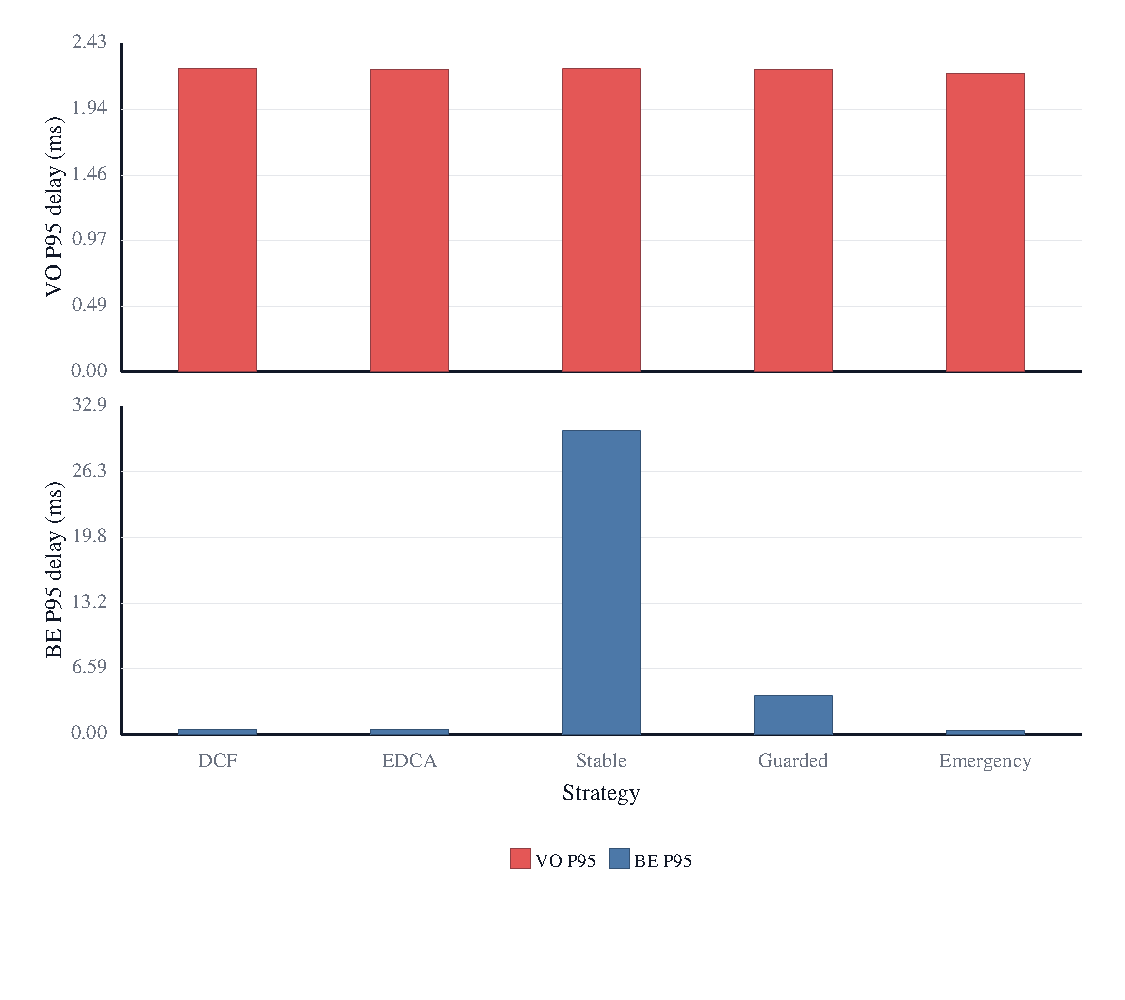
\includegraphics[width=0.92\linewidth, trim=0 50 0 8, clip]{Figs/fig_01_p95_delay_priority_gap_highway_heavy.pdf}
	\end{center}
	\fonte{Prepared by the author.}
\end{figure}

The floor that every policy shares is set by the alert generator itself rather than by channel access.
Each physical copy of a burst---including the first---is dispatched at an offset $\max(0,\,U(-J,\,J))$ after the logical burst timestamp that defines the delay origin, where $J$ is the configured repeat jitter (\autoref{sec:impl:crash}).
That offset therefore has a point mass at zero and a 95th percentile of $0.9\,J$: about \SI{1.8}{\milli\second} at the high-load setting $J=\SI{2}{\milli\second}$ and about \SI{4.5}{\milli\second} at the low and medium setting $J=\SI{5}{\milli\second}$.
Adding the sub-millisecond transfer delay measured on the same samples reproduces the observed floors of about 2.2~ms and 4.6--4.9~ms respectively, and the mean behaves the same way: $\E[\max(0,\,U(-2,2))]=\SI{0.5}{\milli\second}$ accounts for half of the 0.99~ms Voice mean in \autoref{tab:eval:heavy_qos}.
Only when the first copy is lost does the inter-copy gap~$g$ enter, adding one further quantum per missed repeat---the application-level repetition on which robust vehicular broadcast schemes rely~\cite{Robust_Broadcast_Ma,Reliable_Broadcast_Farnoud}.
At the 95th percentile under diffuse load that regime is rare, so contention shifts probability mass within a generator-imposed floor instead of creating a \gls{mac}-policy lever.
Two consequences follow for how the 2.2~ms figure should be read: it is not a pure medium-access measurement, and no MAC policy could have moved it.

%%%%%%%%%%%%%%%%%%%%%%%%%%%%%%%%%%%%%%%%%%%%%%%%%%%%%%%%%%%%%%%%%%%%%%%%%%%%%%%%
\section{The Best Effort Cost of Protection}
\label{sec:eval:cost}

Section~\ref{sec:eval:hotspot} established what emergency preemption \emph{buys} under concentrated load.
This section prices what protection \emph{costs}, starting from the hotspot cell and then noting the same mechanism under uniform load---where there is no Voice return.

\subsection{Hotspot pricing}
\label{sec:eval:cost:hotspot}

At \texttt{hotspot\_high} the Best Effort bill is inseparable from the Voice win.
Emergency drops about $16.1\times10^{3}$ Best Effort frames while blocked (\autoref{tab:eval:hotspot}).
That preemption is also what prevents crash-node Best Effort starvation: under EDCA/\texttt{stable}/\texttt{guarded} the same-sender Best Effort mean reaches $0.98$--$1.45$~\si{\second}, versus 3.3~ms under emergency.
\autoref{fig:eval:gain_cost} places the tradeoff in $\Delta$-space versus plain \gls{dcf}: under hotspot high load, emergency alone moves left on the Voice axis; under uniform high load the adaptive policies buy no Voice P95 reduction while Best Effort P95 rises---especially under \texttt{stable}.

\begin{figure}[htb]
	\caption{\label{fig:eval:gain_cost}Voice-gain versus Best Effort cost relative to plain \glsentryshort{dcf} at high load (three-seed means). Dual panels use independent axes: left is uniform \texttt{netload\_high}; right is \texttt{hotspot\_high}. Negative $\Delta$ Voice P95 is an improvement; positive $\Delta$ Best Effort P95 is a penalty.}
	\begin{center}
		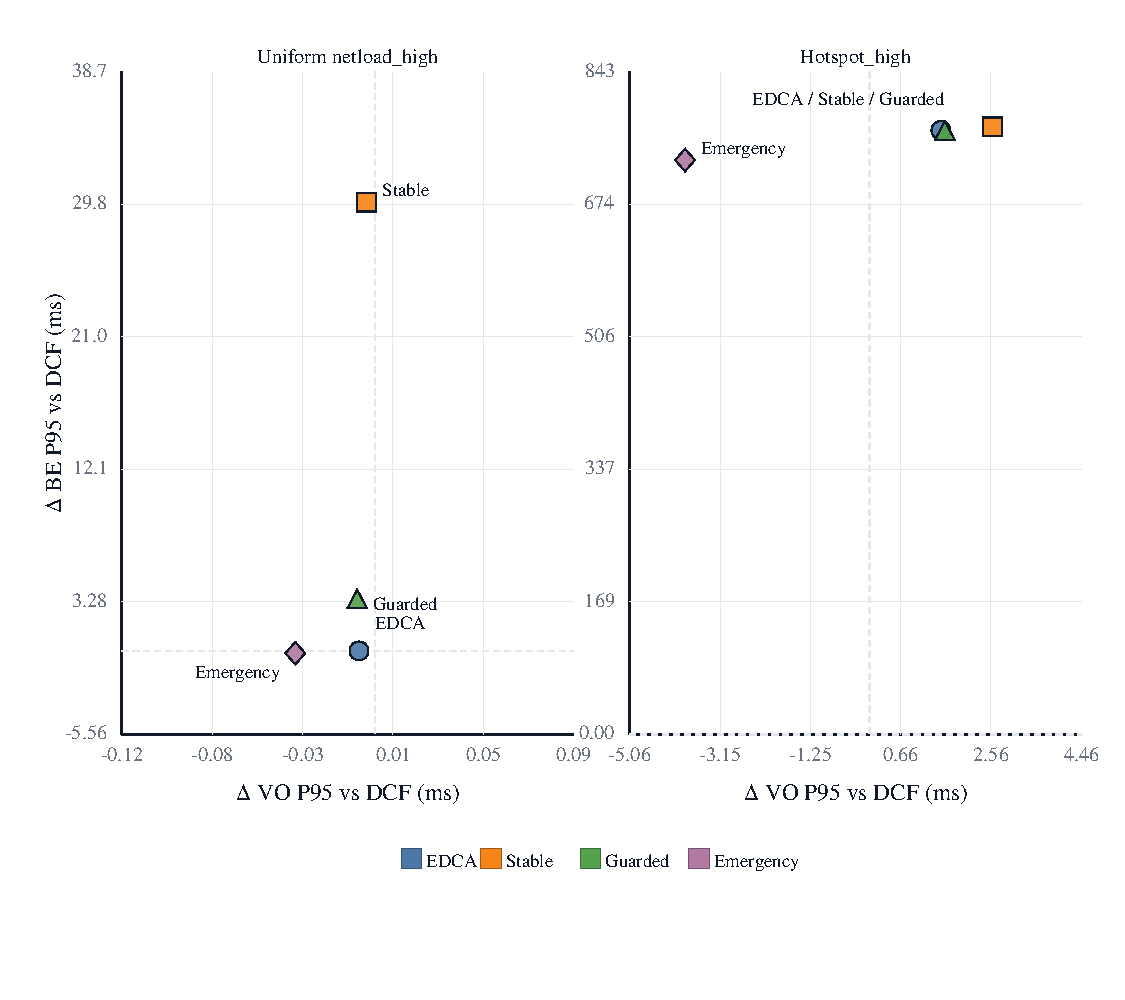
\includegraphics[width=0.95\linewidth, trim=0 50 0 8, clip]{Figs/fig_04_vo_gain_vs_be_cost_highway_heavy.pdf}
	\end{center}
	\fonte{Prepared by the author.}
\end{figure}

\subsection{Uniform-load cost without a Voice target}
\label{sec:eval:heavy:ladder}

Under the uniform matrix the same controller still fires, but without a Voice return (\autoref{tab:eval:heavy_p95}, \autoref{tab:eval:heavy_ctrl}, \autoref{fig:eval:ctrl}).
\texttt{stable} and \texttt{guarded} accumulate about $1.1\times10^{5}$ protection activations per high-load run with zero preemption counters, stretching fleet Best Effort P95 to 30~ms and 3.9~ms.
Emergency pays about $2.5\times10^{3}$ Best Effort drops while blocked plus twelve suppressed grants and keeps fleet and crash-sender tails at 0.37~ms and 0.44~ms---below plain---while Voice P95 remains on the 2.2~ms floor.
In short: deferral buys delay; dropping buys silence; only dropping yields Voice service once a concentrated target exists (\autoref{sec:eval:hotspot}).

\begin{table}[htb]
	\ABNTEXfontereduzida
	\caption{\label{tab:eval:heavy_p95}Best Effort 95th-percentile delay (ms) across offered-load regimes for the five-policy ladder (100~vehicles, three-run means with min--max range across seeds). Voice rows are omitted: Voice P95 stays on the generator's dispatch-jitter floor for every policy (\autoref{sec:eval:light}). Cells with a vanishing seed spread omit the range.}
	\begin{center}
		\scriptsize
		\setlength{\tabcolsep}{3pt}
		\begin{tabularx}{\linewidth}{@{}l *{5}{>{\centering\arraybackslash}X}@{}}
			\toprule
			\textbf{Load} & \textbf{Plain} & \textbf{EDCA} & \textbf{Stable} & \textbf{Guarded} & \textbf{Emerg.} \\
			\midrule
			\multicolumn{6}{@{}l}{\textit{\gls{be} (background, fleet)}} \\
			\texttt{low}    & 0.217 & 0.217 & \shortstack{0.323\\[-1pt]{\scriptsize [0.217--0.419]}} & 0.217 & 0.217 \\
			\texttt{medium} & 0.297 & 0.297 & \shortstack{2.081\\[-1pt]{\scriptsize [0.711--3.203]}} & \shortstack{0.357\\[-1pt]{\scriptsize [0.297--0.387]}} & 0.297 \\
			\texttt{high}   & \shortstack{0.511\\[-1pt]{\scriptsize [0.509--0.513]}} & \shortstack{0.524\\[-1pt]{\scriptsize [0.507--0.538]}} & \shortstack{30.491\\[-1pt]{\scriptsize [27.614--34.175]}} & \shortstack{3.889\\[-1pt]{\scriptsize [2.955--4.458]}} & \textbf{0.369} \\
			\addlinespace
			\multicolumn{6}{@{}l}{\textit{\gls{be} from the crash node}} \\
			\texttt{low}    & 0.217 & 0.217 & \shortstack{0.708\\[-1pt]{\scriptsize [0.641--0.753]}} & \shortstack{1.357\\[-1pt]{\scriptsize [0.217--2.871]}} & 0.217 \\
			\texttt{medium} & 0.297 & \shortstack{0.335\\[-1pt]{\scriptsize [0.297--0.411]}} & \shortstack{3.040\\[-1pt]{\scriptsize [2.419--3.814]}} & \shortstack{2.323\\[-1pt]{\scriptsize [1.197--3.110]}} & 0.297 \\
			\texttt{high}   & \shortstack{0.631\\[-1pt]{\scriptsize [0.621--0.651]}} & \shortstack{0.772\\[-1pt]{\scriptsize [0.731--0.842]}} & \shortstack{13.763\\[-1pt]{\scriptsize [13.541--13.955]}} & \shortstack{3.865\\[-1pt]{\scriptsize [3.769--3.944]}} & \shortstack{\textbf{0.435}\\[-1pt]{\scriptsize [0.369--0.567]}} \\
			\bottomrule
		\end{tabularx}
	\end{center}
	\fonte{Prepared by the author.}
\end{table}

\begin{table}[H]
	\ABNTEXfontereduzida
	\caption{\label{tab:eval:heavy_ctrl}Adaptive-controller actions at heavy-density high load (three-run means; Voice-protection and Best Effort-drop columns in thousands, $\times 10^{3}$; Best Effort hold is a raw event count). The \texttt{emergency} hold entry is about 12 grant-suppression events.}
	\begin{center}
		\small
		\setlength{\tabcolsep}{5pt}
		\begin{tabular}{@{}lrrr@{}}
			\toprule
			\textbf{Policy} &
			\textbf{VO protection} &
			\textbf{BE drop while blocked} &
			\textbf{BE hold} \\
			\midrule
			Stable    & 115  & 0  & 0 \\
			Guarded   & 115  & 0  & 0 \\
			Emergency & 127 & 2.53 & 12 \\
			\bottomrule
		\end{tabular}
	\end{center}
	\fonte{Prepared by the author.}
\end{table}

\begin{figure}[htb]
	\caption{\label{fig:eval:ctrl}Adaptive-controller actions by offered load, heavy density (three panels): Voice-protection activations, Best Effort grants suppressed while blocked, and Best Effort frames dropped while blocked. Emergency alone combines protection with explicit preemption; \texttt{stable} and \texttt{guarded} mainly accumulate protection windows without dropping.}
	\begin{center}
		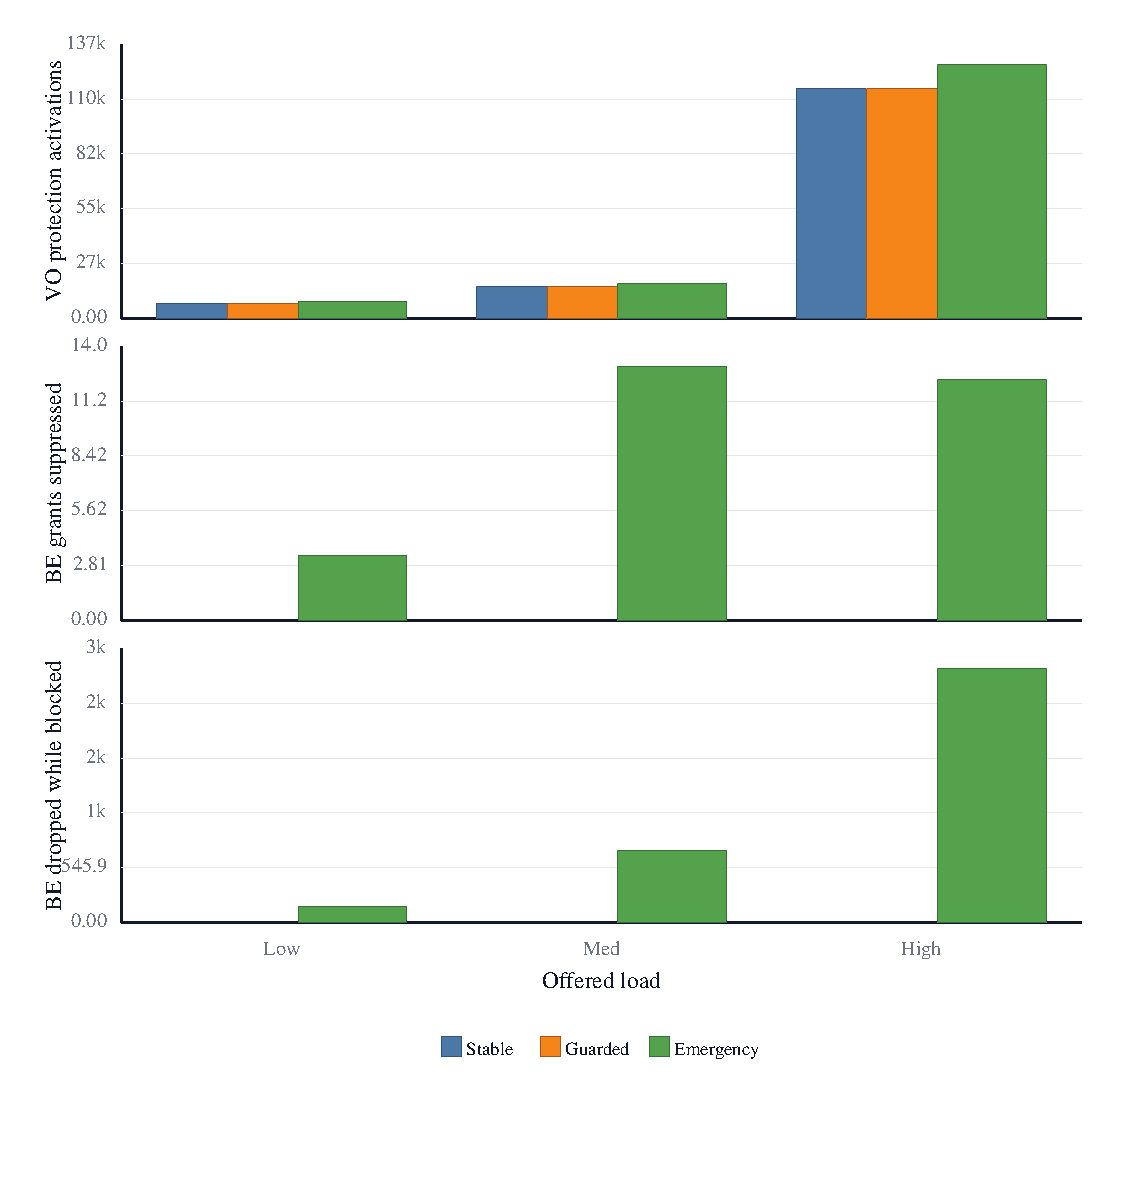
\includegraphics[width=0.88\linewidth, trim=0 50 0 8, clip]{Figs/fig_07_v2x_control_actions_by_load_highway_heavy.pdf}
	\end{center}
	\fonte{Prepared by the author.}
\end{figure}

\section{Discussion}
\label{sec:eval:discussion}

\subsection{Event-triggered escalation, not always-on QoS}
\label{sec:eval:disc:escalation}

Adaptive blocking is harmful when armed without Voice-limited congestion: \texttt{stable} and \texttt{guarded} inflate Best Effort delay while Voice alert age stays put (\autoref{sec:eval:light}).
The mechanism should be treated as an escalation level attached to genuine channel stress, not as an always-on replacement for ordinary EDCA marking~\cite{IEEE80211e_2005,aguiar2026_veins_qos}.
Explicit DSCP-to-Voice mapping remains a reasonable default; bounded or emergency suppression should be reserved for the concentrated regime of \autoref{sec:eval:hotspot}, where preemption flips from pure cost to measured Voice benefit (\autoref{tab:eval:hotspot}).

\subsection{Reading the baseline correctly}
\label{sec:eval:disc:plain}

Two measurement traps are aggregation artifacts rather than policy effects.
First, under \texttt{plain} both classes receive identical per-frame \gls{mac} treatment, yet \autoref{tab:eval:heavy_qos} shows a Voice--Best Effort delay gap: the gap reflects different traffic processes (one crash-node alert stream versus a fleet-wide Poisson offer), not a differentiating \gls{dcf} queue.
Second, Voice RX/alert exceeds Best Effort RX/TX for structural reasons---different denominators and a denser neighborhood around the stopped crash node.
Cross-class comparisons within one policy therefore describe different traffic processes; the crash-node Best Effort slice is the controlled same-sender check, and cross-policy comparisons within one class remain the policy measurement.
Poisson redraws keep Best Effort offer at about 22~thousand transmissions on every uniform run, so seeds no longer split into an uncongested draw and two saturated draws.

\subsection{Regime-conditional significance of the Voice effects}
\label{sec:eval:disc:significance}

Under the uniform matrix there is no Voice-tail reduction to claim against representative V2X latency budgets such as the~\SI{25}{\milli\second} end-to-end bound for cooperative platooning in \gls{threegpp} TS~22.186~\cite{ts22186}: absolute Voice P95 stays near 2.2~ms for every policy (\autoref{sec:eval:light}).
That margin is moreover partly structural rather than earned by the channel, since about \SI{1.8}{\milli\second} of the 2.2~ms is the alert generator's own per-copy dispatch jitter (\autoref{sec:eval:light}); the medium-access contribution to the uniform-load tail is smaller still.
The hotspot cell of \autoref{tab:eval:hotspot} is where absolute tails re-enter that budget band and where emergency compresses them.
Three seeds per cell keep this a mechanism check rather than an effect-size estimate (\autoref{sec:eval:disc:limits}); the boundary itself is the take-home---the same preemption is a cost center under uniform load and a Voice lever under concentrated load.

\subsection{Protection cost, class granularity, and spatial fairness}
\label{sec:eval:disc:cost}

Bounded protection makes Best Effort service worse than plain \gls{dcf} at high uniform load, and emergency converts part of the backlog into explicit loss while keeping the fleet Best Effort tail short (\autoref{sec:eval:cost}).
Because the model treats \emph{all} Best Effort traffic as suppressible, these penalties are a worst-case bound for the two-class abstraction (\autoref{sec:sys:scope}): in a real stack, traffic outside the current crash alert may still be safety relevant.
Deployments would need finer-grained classes before comparable \gls{mac} aggression, and the trade-off is defensible only for genuinely critical, short-lived flows such as the alert window studied here.

\label{sec:eval:disc:spatial}
Nor is the penalty uniform across vehicles: protection is armed locally by overheard Voice frames, so vehicles near the crash source defer or drop Best Effort while distant vehicles continue unaffected (\autoref{sec:sys:controller}).
The Best Effort cost is spatially concentrated around the event---arguably desirable for a crash---but pooled averages understate the worst-affected vehicles; per-vehicle fairness is left as future work.

\subsection{Preemption as a starvation cure under concentrated contention}
\label{sec:eval:disc:starvation}

Under concentrated contention, \gls{edca}-family queues can starve the very node they should serve first.
At \texttt{hotspot\_high}, crash-node Best Effort means of $0.98$--$1.45$~\si{\second} under EDCA/\texttt{stable}/\texttt{guarded} collapse to 3.3~ms under emergency (\autoref{tab:eval:hotspot}).
Dropping is therefore both the Voice lever and the starvation cure when continuous hotspot demand would otherwise own local arbitration.

\subsection{Burst cadence as an online arming trigger}
\label{sec:eval:disc:trigger}

The dose-response of \autoref{tab:eval:hotspot_dose} implies a measurable online signal for deciding when protection is worth its cost: arm emergency suppression only while recent alert cadence times the bounded block window (\autoref{tab:impl:parameters}) saturates the available blocking budget.
The controller already tracks activation count and \texttt{maxContinuousBlock}, so the trigger is an instrumentation problem, not a new measurement.
This closes the escalation design loop of \autoref{sec:eval:disc:escalation}.

\subsection{Denial-of-service risk of Voice-triggered suppression}
\label{sec:eval:disc:dos}

Protection is armed by local Voice queue pressure and \emph{overheard} Voice frames without authenticating the sender, so a faulty or malicious node continuously emitting Voice-marked traffic could keep nearby vehicles in blocking mode.
The risk is bounded but not removed: protection windows are finite (20--80~ms maximum continuous block plus a guard interval, \autoref{tab:impl:parameters}) and suppression affects only a node's own Best Effort transmissions.
Real deployment would additionally require V2X message authentication, rate limiting of alert bursts, and plausibility checks before Voice frames may trigger suppression.

\subsection{Limitations and threats to validity}
\label{sec:eval:disc:limits}

Heavy-density \glspl{kpi} average three seeds and report the min--max range on headline delay tables, still without confidence intervals or significance tests, so results are qualitative mechanism checks rather than proven effect sizes; all observed prioritization is statistical contention shaping, not deterministic real-time communication~\cite{kosekszott2012What}.
The evaluation is simulation-only, models a single crash source on a one-hop highway corridor, and uses the simplified \gls{phy} assumptions of \autoref{chap:implementation} and \autoref{sec:sys:scope}; concurrent alerts would arm overlapping protection windows whose interaction is not evaluated.
Results do not predict absolute performance under richer propagation or congestion control, and no adaptive-EDCA or \gls{dcc} baseline is implemented, so no superiority claim is made against those families~\cite{etsi_dcc_2018}.
The configured \gls{edca} parameters follow the IEEE~802.11 BSS QoS defaults rather than the distinct \gls{ocb} default set, and group-addressed frames use \gls{inet}'s default fastest-mandatory-mode rate selection rather than a basic-rate policy (\autoref{sec:impl:radio}); both choices are uniform across policies but may shift absolute values relative to deployed 802.11p stacks.
The \texttt{high} crash-burst profile is a deliberate stress case rather than a standardized alert schedule, and no application-level safety deadline is evaluated.
The three adaptive profiles are fixed design points whose triggers are not individually ablated, although their spread of block windows (4--15~ms) and Voice thresholds (1--3 packets) acts as a coarse sensitivity ladder; a systematic parameter sweep is future work.
The hotspot cells place streaming nodes by injection order rather than by a received-power map, so the exact gain magnitudes depend on that geometry; the sign of the effect---and its absence at sparser burst cadences---is the claim, not the decimals.
Within that scope the comparison remains internally fair: all configurations share the same \gls{phy} stack, mobility trace, and load matrix, isolating \gls{mac}-policy effects~\cite{aguiar2026_veins_qos}.

%%%%%%%%%%%%%%%%%%%%%%%%%%%%%%%%%%%%%%%%%%%%%%%%%%%%%%%%%%%%%%%%%%%%%%%%%%%%%%%%
\section{Chapter Summary}
\label{sec:eval:summary}

The evaluation compared five \gls{mac} policies on the same highway matrix and found a regime-conditional answer rather than a universal Voice-tail race.
The primary positive result is \texttt{hotspot\_high}: emergency preemption recovers Voice service when near-crash airtime is concentrated and bursts are dense enough to keep protection armed (\autoref{tab:eval:hotspot}).
The uniform Poisson matrix is the null that makes that result conditional: Voice alert age stays on the generator's dispatch-jitter floor for every policy, while adaptive blocking mainly taxes Best Effort (\autoref{sec:eval:light}).
Bounded blocking without dropping (\texttt{stable}, \texttt{guarded}) never converts hotspot stress into Voice service; dropping is the load-shedding step that both compresses the Voice tail and cures crash-node Best Effort starvation.
The practical takeaway is therefore conditional: explicit DSCP-to-Voice marking is a reasonable default; adaptive blocking---especially emergency preemption---is justified as an event-triggered escalation where near-crash congestion is concentrated, with authentication and rate limiting as deployment prerequisites.

The subsequent chapter concludes the dissertation by summarizing these findings, stating the conditional practical takeaway, and outlining limitations and future work.
